\documentclass{article}
\usepackage{listings}
\usepackage{mathrsfs}
\usepackage[utf8]{inputenc}
\usepackage{amssymb}
\usepackage{lipsum}
\usepackage{amsmath}
\usepackage{fancyhdr}
\usepackage{geometry}
\usepackage{scrextend}
\usepackage[english,german]{babel}
\usepackage{titling}
\usepackage{verbatim}
\setlength{\droptitle}{-3cm}
\usepackage{tikz}
\usepackage{algorithm,algpseudocode}
\usepackage[doublespacing]{setspace}
\usetikzlibrary{datavisualization}
\usetikzlibrary{datavisualization.formats.functions}
\usepackage{polynom}
\usepackage{amsmath}
\usepackage{gauss}
\usepackage{euscript}
\usepackage{tkz-euclide}
\usepackage{stackengine}
\usetikzlibrary{datavisualization}
\usetikzlibrary{datavisualization.formats.functions}
\title{Übungsblatt 5}
\author{
Alexander Mattick Kennung: qi69dube}
\usepackage{import}
\date{\today}
\geometry{a4paper, margin=2cm}
\usepackage{stackengine}
\parskip 1em
\newcommand\stackequal[2]{%
  \mathrel{\stackunder[2pt]{\stackon[4pt]{=}{$\scriptscriptstyle#1$}}{%
  $\scriptscriptstyle#2$}}
 }
\makeatletter
\renewcommand*\env@matrix[1][*\c@MaxMatrixCols c]{%
  \hskip -\arraycolsep
  \let\@ifnextchar\new@ifnextchar
  \array{#1}}
\makeatother
\lstset{
  language=haskell,
}
\lstnewenvironment{code}{\lstset{language=Haskell,basicstyle=\small}}{}
\usepackage{enumitem}
\setlist{nosep}
\usepackage{titlesec}
\newcommand{\nto}{\nrightarrow}
\newcommand{\smallAscr}{\scriptscriptstyle\mathcal{A}}
\title{Erläuterung monotonie}
\titlespacing*{\subsection}{0pt}{2pt}{3pt}
\titlespacing*{\section}{0pt}{0pt}{5pt}
\titlespacing*{\subsubsection}{0pt}{1pt}{2pt}
\newtheorem{satz}{Satz}
\newtheorem{korrolar}{Korrolar}[section]
\newtheorem{lemma}{Lemma}[section]
\newtheorem{beweis}{Beweis}[section]
\newtheorem{beispiel}{Beispiel}[section]
\newtheorem{definition}{Definition}[section]
\setcounter{section}{2}
\usepackage{ marvosym }
\begin{document}
	\maketitle\noindent
	Konstruieren wir ein Gegenbeispiel:\\
	Sei $a_n = (-1)^n\cdot n$ also $-1,2,-3,4,-5,\dots$\\
	Machen wir also einen Widerspruchsbeweis, dass der Widerspruchsbeweis funktioniert.\\
	\textbf{Annahme: ein Widerspruchsbeweis funktioniert.}\\
	Dafür nehmen wir einfach monoton steigend $\frac{a_{n+1}}{a_n} \geq 1$ an.\\
	wir erhalten $\frac{a_{n+1}}{a_n}\geq 1 \iff \frac{(-1)^{n+1}\cdot (n+1)}{(-1)^n\cdot n}\geq 1 \stackon{$\iff$}{$\scriptscriptstyle\text{kürzen}(-1)^n$}{} \frac{(-1)\cdot (n+1)}{n}\geq 1\iff \frac{-n-1}{n} \geq 1\iff \frac{-n}{n}-\frac{1}{n} \geq 1\iff -1+\frac{1}{n}\geq 1\iff \bot \forall n\in\mathbb{N}$\\
	aus dem Widerspruch folgern wir: $a_n$ ist monoton wachsend.\\
	Das ist aber offensichtlich falsch: $a_2=2> a_3=-3$.\\
	\textbf{Dies ist ein Widerspruch dazu, dass ein Widerspruchsbeweis funktioniert.} (analog wenn man monoton fallend annimmt)\\
	Das Problem mit dem Widerspruchsbeweis ist, dass ein Widerspruchsbeweis immer davon ausgeht, dass es zwei Zustände gibt, die sich beide gegenseitig ausschließen: z.B. ``alle Werte dieser Funktion sind gerade'' es gibt entweder ``Wahr'' oder ``Falsch''.\\
	Im Fall der Monotonie gibt es aber \textbf{3 Fälle: monoton wachsend, monoton fallend und keins von beiden!}\\
	Aus ``nicht monoton wachsend'' folgt entweder ``monoton fallend'' oder ``keine Monotonie''. Welches von beiden das ist kann man nur aus ``nicht monoton wachsend'' nicht rausfinden.\\
	\[\lnot \text{``monoton steigend''} \implies \text{``nicht monoton wachsend''}\oplus\text{``keine Monotonie''}\]
	Das hab ich auch versucht mit der Funktion zu zeigen: $f(x)=(x-3)^2(x+1)$ sieht so aus\\
	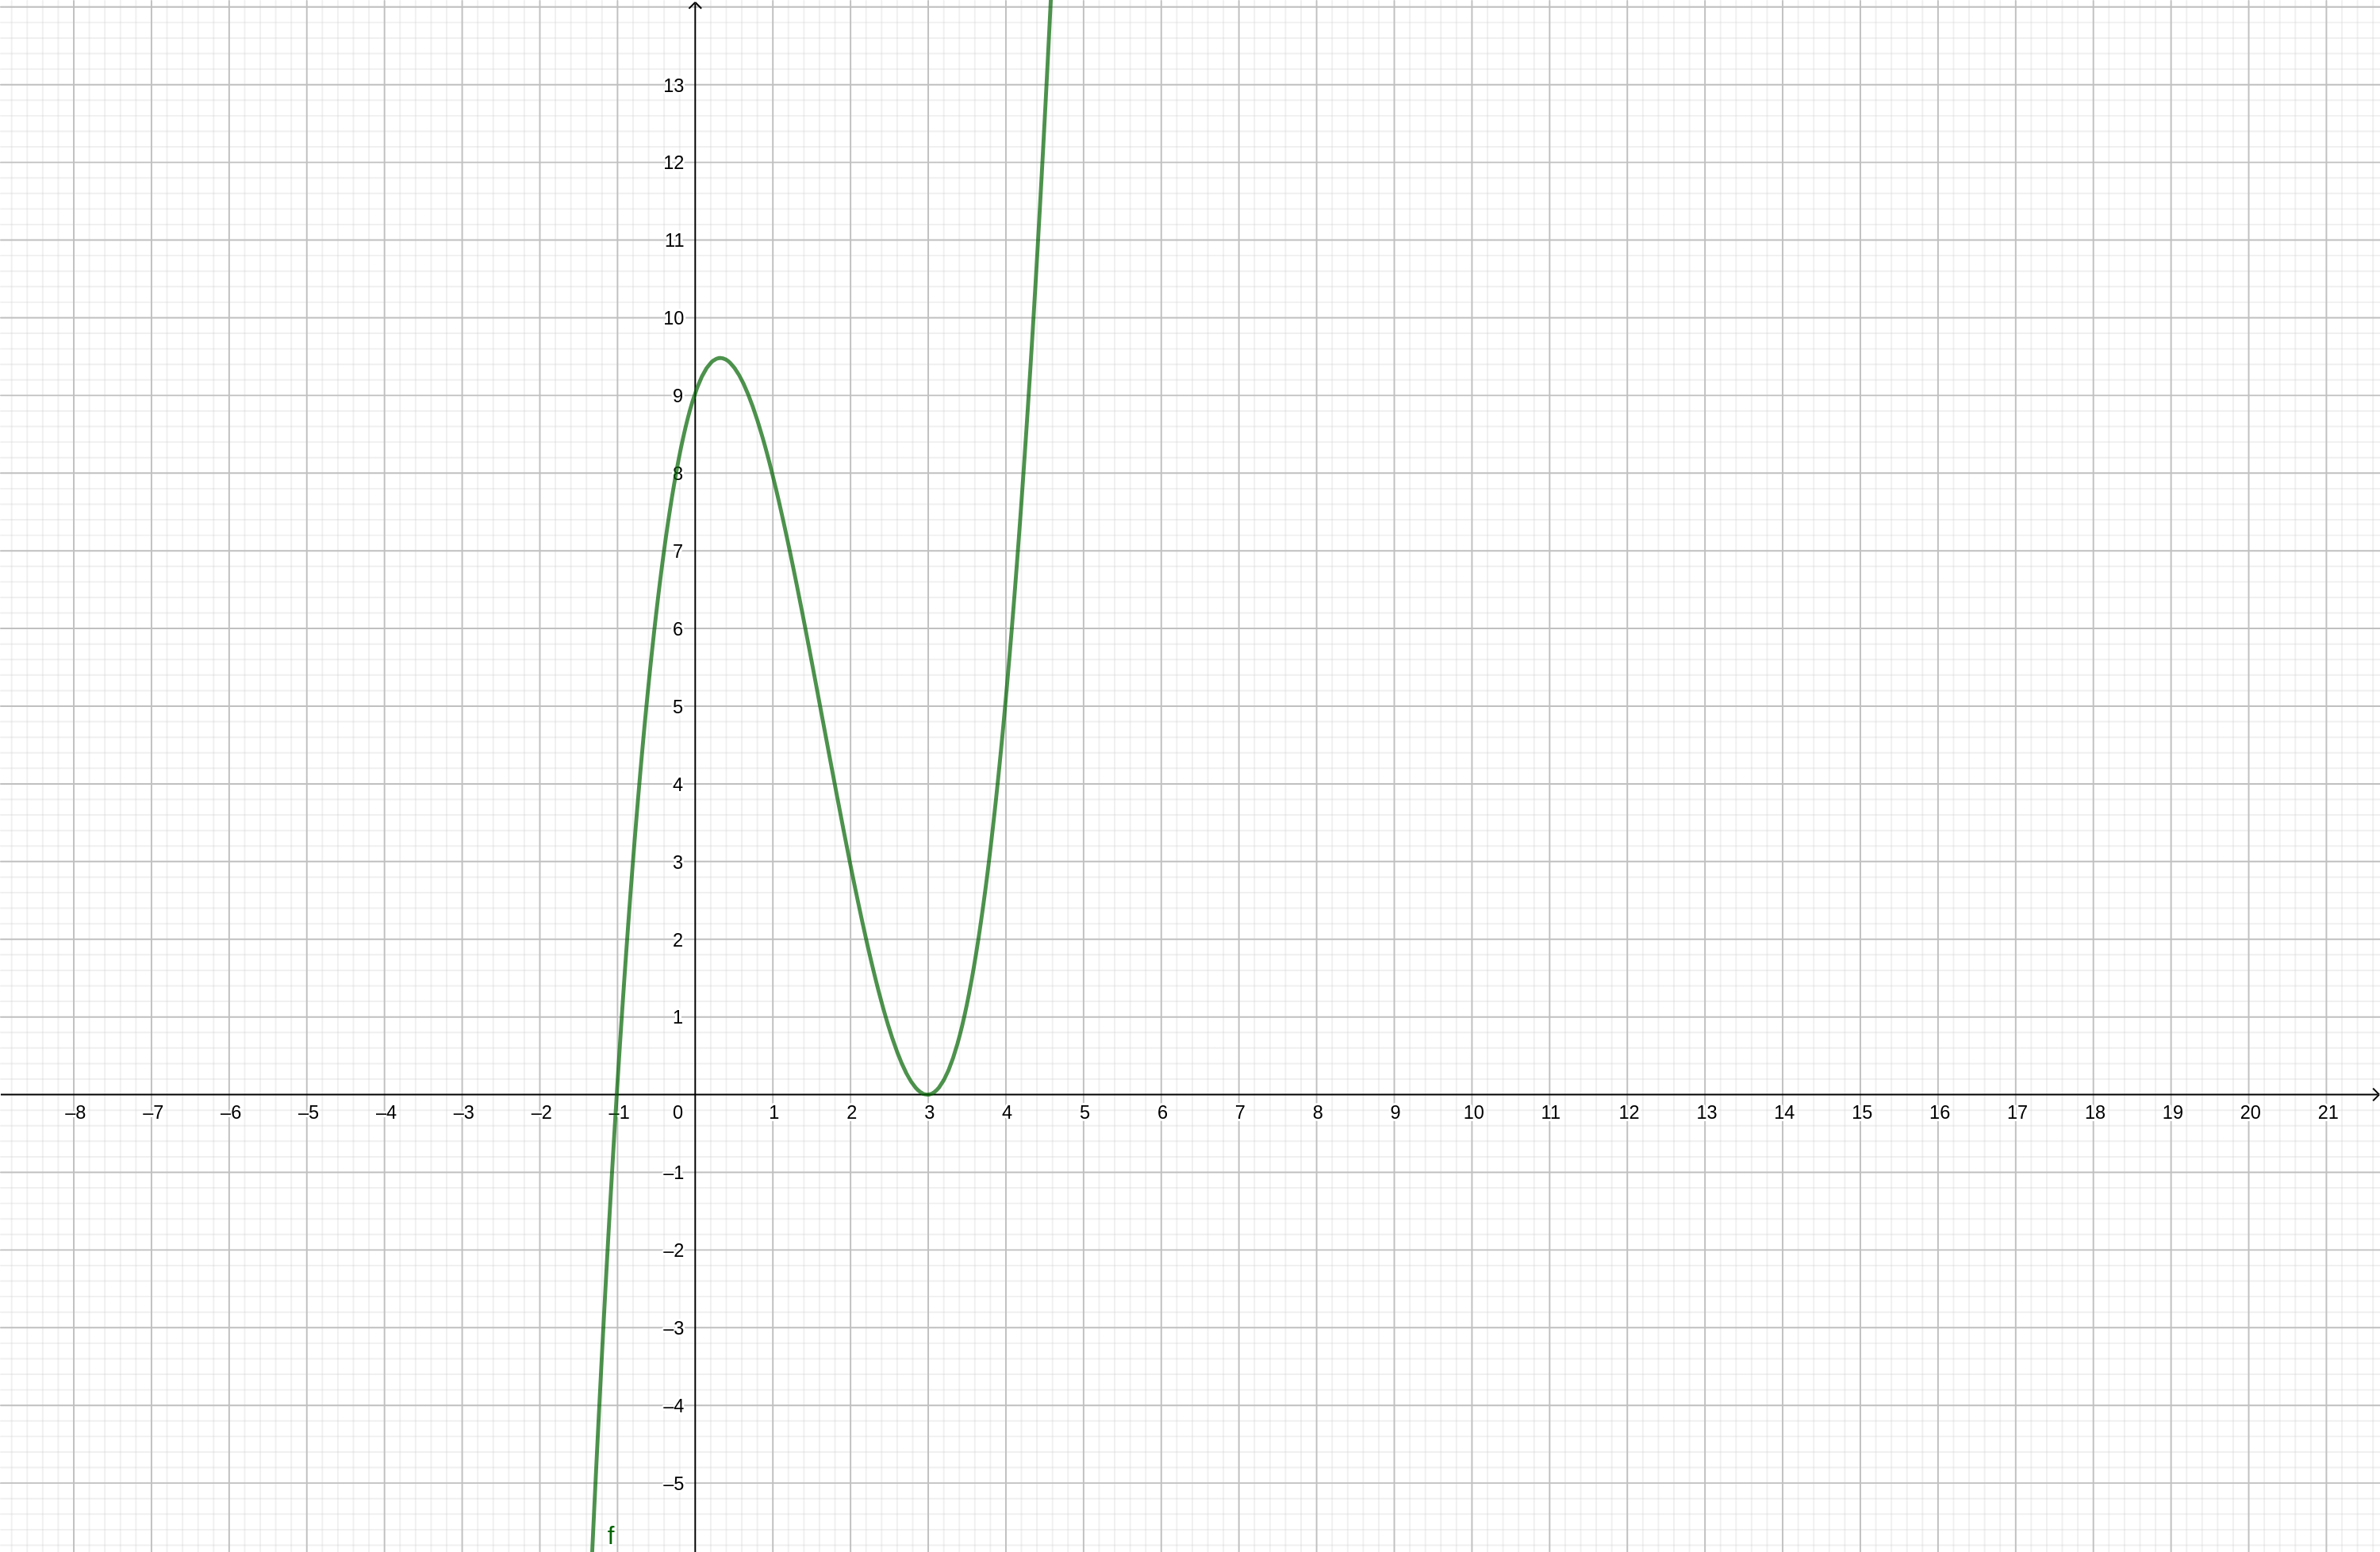
\includegraphics[width=150px]{images/montonie.png}\\
	Wenn man hier versucht allgemein streng monoton steigend zu beweisen, schlägt das offensichtlich fehl.\\
	$(x+1-3)^2(x+1+1) - (x-3)^2(x+1) \geq 0\iff 3x^2-7x-1\geq 0 \iff \bot$ für z.B. $x=1$\\
	heißt das jetzt das $f(x)$ streng monoton fällt?\\
	Auf logischer Ebene ist das Problem vielleicht etwas Eindeutiger, wenn man Monotonie von Folgen einmal formal aufschreibt:\\
	$\forall n\in \mathbb{N}: a_{n+1}>a_{n}$ (ersetz $>$ mit $<,\leq,\geq$ für die anderen monotonien)\\
	Dein Widerspruchsbeweis will jetzt $\lnot \forall n\in \mathbb{N}: a_{n+1}>a_{n}$ zeigen.\\
	Umformen liefert: $\lnot\forall n\in \mathbb{N}: a_{n+1}>a_{n}\iff\exists n\in \mathbb{N}:\lnot( a_{n+1}>a_{n}) \iff \exists n\in \mathbb{N}:\lnot( a_{n+1}\leq a_{n})$\\
	Also in Worten: monoton steigend heißt, dass der Nachfolger größer als der vorgänger ist.\\
	nicht monoton steigend heißt, dass es mindestens einen gibt, für den dies nicht gilt.\\
	(ein einziges n das nicht steigt macht ein $\forall$ schon kaputt\dots)\\
	Monoton fallend heißt aber, dass für alle n diese Aussage nicht gilt.\\
	$\forall n\in \mathbb{N}: \lnot ( a_{n+1}>a_{n}) \iff \forall n\in \mathbb{N}:( a_{n+1}\leq a_{n})$\\
\end{document}





